\section{Small eigenvalues of the endomorphism Laplacian}\label{sec:spectrum}

All operators in this section are evaluated at the reference metric $h_0$.
Put $L=\log(1/|t|)$ and let
\[
 \mathcal L_{t,\theta}=D_\theta^*D_\theta
 \quad\hbox{on }\Herm_0(\cB_{t,\theta}).
\]
The subscript zero denotes trace-free, $h_0$-Hermitian endomorphisms.
We use the unnormalized trace norm and the nonnegative connection
Laplacian. This operator is the negative infinitesimal generator of
determinant-normalized HYM metric flow at $h_0$. Indeed expansion of
the Chern metric equation at $h_0e^{\Psi}$ gives
$\Psi_s=-D_\theta^*D_\theta\Psi$ to first order; the contracted background
curvature commutator vanishes because $i\Lambda F_{D_\theta}=0$.
The operator is not a Yang--Mills Hessian on connection one-forms.

Write $e_x=\sigma_x/\sqrt2$, $e_y=\sigma_y/\sqrt2$ and
$e_z=\sigma_z/\sqrt2$, where
$\sigma_y=\left(\begin{smallmatrix}0&-i\\i&0\end{smallmatrix}\right)$.
These form an orthonormal real basis of $\Herm_0(2)$. Define
\begin{equation}\label{eq:five-forms}
 \begin{split}
 q_\theta(a,X,b)&=2\bigl(\|au-X\|^2+\|X-bv_\theta\|^2\bigr),\\
 m_A(a,X,b)&=A_0a^2+2A_1\|X\|^2+A_2b^2,\\
 u&=(1,0,0),\qquad v_\theta=(\cos\theta,\sin\theta,0),
 \end{split}
\end{equation}
on $\RR\oplus\RR^3\oplus\RR$. Denote their generalized eigenvalues
by $0\le\mu_0(\theta)\le\cdots\le\mu_4(\theta)$, including zeros.

\begin{theorem}\label{thm:five-spectrum}
There are $\gamma>0$ and $\varepsilon(t)\to0$ as $t\to0$ such that
the eigenvalues of $\mathcal L_{t,\theta}$ satisfy
\begin{equation}\label{eq:five-relative}
 (1-\varepsilon(t))\frac{2\pi}{L}\mu_k(\theta)
 \le\lambda_k(t,\theta)\le
 (1+\varepsilon(t))\frac{2\pi}{L}\mu_k(\theta)
 \quad(0\le k\le4),\qquad \lambda_5(t,\theta)\ge\gamma.
\end{equation}
The estimates are uniform in the unitary parameter. For small $t$ there
are exactly five eigenvalues below a fixed positive threshold, counting
zero modes. The kernel has dimension one when $\theta\in\pi\ZZ$ and
zero otherwise. No relation between $t$ and the distance of $\theta$
to $\pi\ZZ$ is required.
\end{theorem}

The spectral reduction uses an exact product decomposition followed by
an equivariant curve estimate. The first step removes every mode which
is nonparallel in the K3 direction. The second step must preserve the
fixed-point constraints at the two ends of the quotient interval.

\subsection{The K3 complement and the quotient normalization}
On the cover the bundle connection is
$D_S\otimes I+I\otimes D_V$. A product orthonormal frame gives the
exact sum decomposition of its endomorphism connection Laplacian.
There are no mixed terms in the energy $\int|D\Phi|^2$.
Let $\Pi_S$ be projection onto the parallel tangent endomorphisms in
the $S$ variable. By \eqref{eq:k3-volume} it is
\begin{equation}\label{eq:k3-projection}
 \Pi_S\Phi=I_{T^{1,0}S}\otimes
 \frac12\int_S\tr_{T^{1,0}S}\Phi\,dV_S.
\end{equation}
The resulting multiplicity endomorphism is Hermitian and trace-free
when $\Phi$ is. The orthogonal complement includes nonconstant scalar
functions on $S$ as well as nonscalar tangent endomorphisms.
The fixed compact K3 connection Laplacian has a positive gap $\gamma_S$
on this entire complement. Apply its inequality at every elliptic point
and integrate. The elliptic energy is nonnegative, so the product
operator is bounded below by $\gamma_S$ on $\ker\Pi_S$, independently
of $t$ and $\theta$.

The deck action preserves the metric and connection and commutes with
$\Pi_S$. The quotient operator is the restriction to invariant sections;
both norm and energy on the cover are divided by two. On the tangent-scalar
sector this division cancels the rank-two tangent factor:
\begin{equation}\label{eq:norm-cancellation}
 \|I_{T^{1,0}S}\otimes f\|_{L^2(X_t)}^2
 =\frac12\|I_{T^{1,0}S}\|^2\operatorname{Vol}(S)
       \int_{E_t}\|f\|^2\,dA
 =\int_{E_t}\|f\|^2\,dA.
\end{equation}
The same identity holds for the energy. It remains to determine the
curve spectrum in this invariant trace-free multiplicity sector.

\subsection{The five-dimensional invariant space}
In component frames an invariant tuple obeys
\begin{equation}\label{eq:linear-invariance}
 X_{-j}=\Ad(J)X_j.
\end{equation}
The fixed subspace of $\Ad(J)$ in $\Herm_0(2)$ is $\RR e_x$.
Thus $X_0=ae_x$, $X_2=be_x$, and $X_3=\Ad(J)X_1$.
There are exactly five real degrees of freedom, with mass
$A_0a^2+2A_1\|X_1\|^2+A_2b^2$.

The transported four-cycle energy is
\[
 q(X_\bullet)=\sum_{j\bmod4}
       \|X_{j+1}-\Ad(R)X_j\|^2.
\]
Using $JR=R^{-1}J$ and \eqref{eq:linear-invariance}, its opposite
terms are equal, giving
\[
 q(X_\bullet)=2\bigl(\|X_1-\Ad(R)X_0\|^2
                         +\|X_2-\Ad(R)X_1\|^2\bigr).
\]
Set $X=\Ad(R^{-1})X_1$. This orthogonal change of middle coordinates
turns the endpoint directions into $u=e_x$ and
$v_\theta=\Ad(R^{-2})e_x=(\cos\theta,\sin\theta,0)$.
It gives exactly \eqref{eq:five-forms}. In particular, the interval
obtained by quotienting the cycle has endpoint \emph{lines} whose
relative angle depends on the gluing. Replacing it by a scalar interval
Laplacian would discard that information.

\begin{figure}[htbp]
\centering
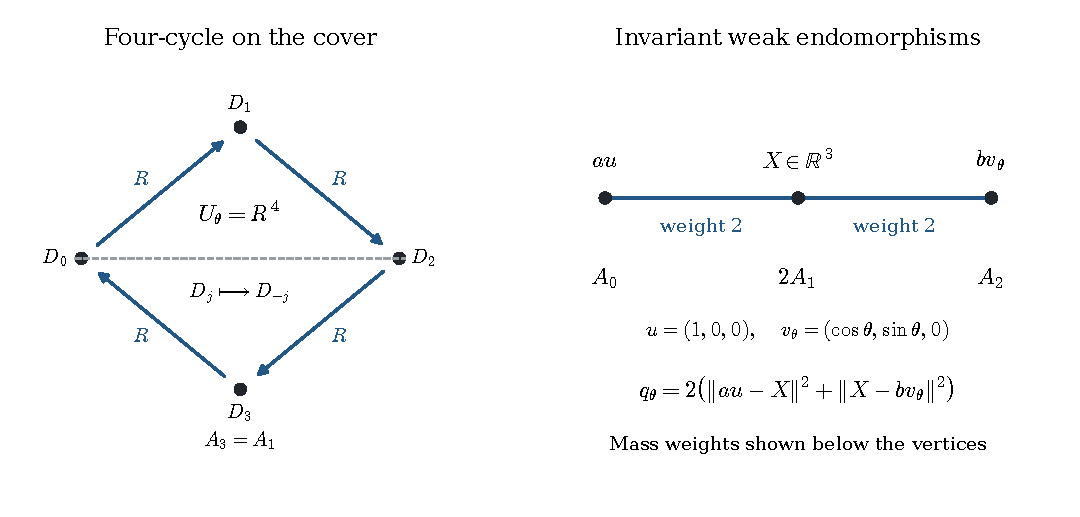
\includegraphics[width=\textwidth]{figures/output/gluing-constraints.pdf}
\caption{The four-cycle on the elliptic cover and its invariant
endomorphism problem. After an orthogonal change of middle frame,
the endpoint lines are $\RR u$ and $\RR v_\theta$.
The two edge coefficients are $2$, and the mass weights are
$A_0,2A_1,A_2$. The diagram represents the exact effective forms
\eqref{eq:five-forms}, not a numerical approximation of the HYM flow.}
\label{fig:gluing-constraints}
\end{figure}

\subsection{Equivariant capacity and mass estimates}
We record the curve estimates needed for the restriction to invariant
sections. Their constants concern the fixed elliptic family and a finite
number of component frames, and are uniform in the unitary transitions.
For a fixed small cutoff radius $a$, take paired node discs and invariant
component exteriors. A section with vertex values $X_j$ is extended by
affine interpolation in $\log|u|$ across a node annulus.
Conformal invariance of two-dimensional Dirichlet energy gives
\begin{equation}\label{eq:curve-trial}
 E(J_tX)=\frac{2\pi}{L+2\log a}\,q(X),\qquad
 \bigl|\|J_tX\|^2-m_A(X)\bigr|
       \le(Ca^2+o_a(1))m_A(X).
\end{equation}
Here $E(f)=\int_{E_t}|D_Vf|^2\,dA$, and $o_a(1)$ tends to zero
as $t\to0$ for fixed $a$. The mass error follows from convergence on
the component exteriors and the node-area bound $O(a^2)$.

Both trial interpolation and component averaging commute with the
involution. At a reflected node the logarithmic coordinate reverses,
and the two endpoints are transported by the verified unitary lift.
On a fixed component, averaging commutes with its isometry and the
constant frame map $J$. Consequently \eqref{eq:curve-trial} restricts
to the five-dimensional space \eqref{eq:linear-invariance}.

For a section $f$, let $b_j(f)$ be its mean on a fixed truncated
component. Poincar\'e and trace inequalities on that fixed component
bound the difference between $b_j(f)$ and the circular mean at an
incident boundary by $C_aE(f)^{1/2}$. Angular averaging and radial
Cauchy--Schwarz on the annulus then give
\begin{equation}\label{eq:curve-lower}
 q(b(f))^{1/2}
 \le\left(\sqrt{\frac{L+2\log a}{2\pi}}+C_a\right)E(f)^{1/2}.
\end{equation}
This is an estimate by the section's own energy, not an additive error
which could dominate a small positive eigenvalue.

For completeness, the mass estimate excluding extra weak modes is
\begin{equation}\label{eq:curve-mass}
 \bigl|m_A(b(f))-\|f\|^2\bigr|
 \le(Ca^2+C_a\sqrt\Lambda+o_a(1))\|f\|^2
\end{equation}
on a span of at most six eigensections with eigenvalues at most
$\Lambda\le1$. On fixed component collars, Poincar\'e and interior
elliptic estimates bound the boundary oscillation around the component
mean by $C_a\sqrt\Lambda$ for an orthonormal eigensection. Their
constants are uniform because the local flat equation and metric have
uniform fixed-chart bounds. The corresponding statement for a combination
of at most six eigensections follows by Cauchy--Schwarz.

On each annulus let $v$ be the harmonic section with the same boundary
values as $f$. The maximum principle controls $v$ by those boundary
values, and its mass is $O(a^2)$ times their squared bound.
The difference $f-v$ has zero boundary values and satisfies
\[
 \int_{\text{annulus}}|f-v|^2\,dA
       \le Ca^2\int_{\text{annulus}}|D_V(f-v)|^2\,dA
       \le Ca^2E(f).
\]
To obtain the first inequality uniformly in the annulus modulus,
use $F=|u|^2+|v|^2$ on the Euclidean curve $uv=t$.
Its divergence Laplacian is four and $|\nabla F|\le Ca$.
Integration by parts against the squared norm of a zero-boundary
section and Cauchy--Schwarz prove the inequality. The actual induced
metric is uniformly comparable to this metric, and Dirichlet energy
is conformally invariant. The second inequality follows from the
Dirichlet orthogonality of $v$ and $f-v$. Summing these bounds with
the component mass estimate proves \eqref{eq:curve-mass}. Invariant
sections have invariant means, so this estimate also restricts to
the required sector.

\begin{proof}[Proof of Theorem~\ref{thm:five-spectrum}]
The invariant trial map and min--max give five eigenvalues of order
$O(L^{-1})$ and their relative upper bounds. If a sixth invariant
curve eigenvalue tended to zero, choose $a$ small and then $t$ small.
Equation~\eqref{eq:curve-mass} would make the averaging map injective
from a six-dimensional spectral space into the five-dimensional
invariant tuple space, a contradiction. The invariant curve complement
therefore has a uniform positive gap $\gamma_E$.

Apply \eqref{eq:curve-lower} and \eqref{eq:curve-mass} on each initial
low spectral subspace and use finite-dimensional min--max. Along with
\eqref{eq:curve-trial}, they give the relative lower and upper bounds.
First fix $a$ for a prescribed error and then take $t$ small. This
produces one function $\varepsilon(t)\to0$ uniform in $\theta$;
no small effective eigenvalue is divided out in any estimate.

The product decomposition and \eqref{eq:norm-cancellation} transfer
these five eigenvalues to the threefold with the same coefficient.
Every other mode has lower bound
$\gamma=\min\{\gamma_S,\gamma_E\}$ after reducing it if necessary.
Finally zero energy means a compatible parallel tuple. In
\eqref{eq:five-forms} this is the equation $X=au=bv_\theta$,
which has one-dimensional solution space when $\sin\theta=0$ and
only the zero solution otherwise. It agrees with
\eqref{eq:parallel-algebra}, proving the exact kernel assertion.
\end{proof}

\begin{corollary}\label{cor:complement}
Let $\Pi_{t,\theta}$ be the orthogonal projection onto the five weak
eigenspaces, counting their exact kernel. On its orthogonal complement,
\[
 \|\mathcal L_{t,\theta}^{-1}(I-\Pi_{t,\theta})\|_{L^2\to L^2}
 \le\gamma^{-1},\qquad
 \|e^{-s\mathcal L_{t,\theta}}(I-\Pi_{t,\theta})\|_{L^2\to L^2}
 \le e^{-\gamma s}.
\]
For $z\notin[\gamma,\infty)$, the complementary resolvent has norm
at most $\operatorname{dist}(z,[\gamma,\infty))^{-1}$.
\end{corollary}

\begin{proof}
Apply the spectral theorem to the nonnegative self-adjoint operator
on the complementary subspace.
\end{proof}

These are $L^2$ estimates in the actual bundle metric. They do not
assert uniform global Schauder bounds across the degenerating necks.
